% !Mode:: "TeX:UTF-8"
\def\usewhat{dvipdfmx}                              % 定义编译方式 dvipdfmx 或者 pdflatex ,默认为 dvipdfmx
                                                    % 方式编译,如果需要修改,只需改变花括号中的内容即可。
%\setlength{\baselineskip}{20pt}
%\setlength{\headheight}{25pt}
\documentclass[a4paper,12.5pt,openany,twoside]{book}

                                           % 如果论文超过60 页 可以使用twoside 双面打印
% !Mode:: "TeX:UTF-8"
%  Authors: 杜家宜   Jiayi Du: Max_dujiayi@gmail.com     湖南大学2010级计算机科学与技术专业博士生

%%%%%%%%%% Package %%%%%%%%%%%%
\usepackage{array}
\newcommand{\PreserveBackslash}[1]{\let\temp=\\#1\let\\=\temp}
\newcolumntype{C}[1]{>{\PreserveBackslash\centering}p{#1}}
\newcolumntype{R}[1]{>{\PreserveBackslash\raggedleft}p{#1}}
\newcolumntype{L}[1]{>{\PreserveBackslash\raggedright}p{#1}}

\usepackage[section]{algorithm}
\usepackage{algorithmic}
\renewcommand{\algorithmicrequire}{\textbf{Input:}}
\renewcommand{\algorithmicensure}{\textbf{Output:}}
\renewcommand{\algorithmiccomment}[1]{\hfill /* #1 */}

%\usepackage{fontspec}
\usepackage{courier}
%\usepackage{enumerate}

\usepackage{graphicx}                       % 支持插图处理
\usepackage{geometry}
\geometry{left=2.5cm,right=2.5cm,top=2cm,bottom=2.5cm,footskip=1.1cm,headsep=0.7cm,head=0.4cm}
                                            % 支持版面尺寸设置
\usepackage{titlesec}                       % 控制标题的宏包
\usepackage{titletoc}                       % 控制目录的宏包
\usepackage{fancyhdr}                       % fancyhdr宏包 支持页眉和页脚的相关定义
\usepackage[UTF8]{ctex}                     % 支持中文显示
\usepackage{color}                          % 支持彩色
\usepackage[table,xcdraw]{xcolor}
\usepackage{amsmath}                        % AMSLaTeX宏包 用来排出更加漂亮的公式
\usepackage{amssymb}                        % 数学符号生成命令
\usepackage[below]{placeins}                %允许上一个section的浮动图形出现在下一个section的开始部分,还提供\FloatBarrier命令,使所有未处理的浮动图形立即被处理
\usepackage{flafter}                        % 使得所有浮动体不能被放置在其浮动环境之前,以免浮动体在引述它的文本之前出现.
\usepackage{multirow}                       % 使用Multirow宏包,使得表格可以合并多个row格
\usepackage{booktabs}                       % 表格,横的粗线;\specialrule{1pt}{0pt}{0pt}
\usepackage{longtable}                      % 支持跨页的表格。
\usepackage{tabularx}                       % 自动设置表格的列宽
\usepackage{setspace}
\usepackage{subfigure}                      % 支持子图 %centerlast 设置最后一行是否居中
\usepackage[subfigure]{ccaption}            % 支持子图的中文标题
\usepackage[sort&compress,numbers]{natbib}  % 支持引用缩写的宏包
\usepackage{enumitem}                       % 使用enumitem宏包,改变列表项的格式
\usepackage{calc}                           % 长度可以用+ - * / 进行计算
\usepackage{txfonts}                        % 字体宏包
\usepackage{bm}                             % 处理数学公式中的黑斜体的宏包
\usepackage[amsmath,thmmarks,hyperref]{ntheorem}  % 定理类环境宏包,其中 amsmath 选项用来兼容 AMS LaTeX 的宏包
\usepackage{CJKnumb}                        % 提供将阿拉伯数字转换成中文数字的命令
\usepackage{indentfirst}                    % 首行缩进宏包
\usepackage{CJKutf8}                        % 用在UTF8编码环境下,它可以自动调用CJK,同时针对UTF8编码作了设置。
\usepackage{CJK}
\usepackage{fancyhdr}
\usepackage{lastpage}
\usepackage{layout}
\usepackage[titles,subfigure]{tocloft}                       %控制生成的表格和图片的目录格式

%\usepackage{hypbmsec}                      % 用来控制书签中标题显示内容

%如果您的pdf制作中文书签有乱码使用如下命令,就可以解决了
\usepackage[dvipdfm, unicode,               % pdflatex, pdftex 这里决定运行文件的方式不同
            pdfstartview=FitH,
            %CJKbookmarks=true,
            bookmarksnumbered=true,
            bookmarksopen=true,
            colorlinks=true,
            pdfborder={0 0 1},
            citecolor=black,
            linkcolor=black,
            anchorcolor=black,
            urlcolor=black,
            breaklinks=true
            ]{hyperref}


                      % 定义本文所使用宏包
\graphicspath{{figures/}}                  % 定义所有的.eps 文件在figures 子目录下


\begin{document}                           % 开始全文
\begin{CJK*}{UTF8}{song}                   % 开始中文字体使用
% !Mode:: "TeX:UTF-8"
%\setCJKfamilyfont{hwhp}{华文琥珀}
%\newcommand{\hwhp}{\CJKfamily{hwhp}}
%\newfontfamily\tempus{Tempus Sans ITC}

%%%%%%%%%% Fonts Definition and Basics %%%%%%%%%%%%%%%%%
\newcommand{\song}{\CJKfamily{song}}    % 宋体
\newcommand{\fs}{\CJKfamily{fs}}        % 仿宋体
\newcommand{\kai}{\CJKfamily{kai}}      % 楷体
\newcommand{\hei}{\CJKfamily{hei}}      % 黑体
\newcommand{\li}{\CJKfamily{li}}        % 隶书

%\setCJKfamilyfont{hwhp}{华文琥珀}
%\newcommand{\hwhp}{\CJKfamily{hwhp}}

%\newfontfamily\tempus{Tempus Sans ITC}

\newcommand{\yihao}{\fontsize{26pt}{26pt}\selectfont}       % 一号, 1.倍行距
\newcommand{\xiaoyi}{\fontsize{24pt}{24pt}\selectfont}      % 小一, 1.倍行距
\newcommand{\erhao}{\fontsize{22pt}{22pt}\selectfont}       % 二号, 1.倍行距
\newcommand{\xiaoer}{\fontsize{18pt}{18pt}\selectfont}      % 小二, 单倍行距
\newcommand{\sanhao}{\fontsize{16pt}{16pt}\selectfont}      % 三号, 1.倍行距
\newcommand{\xiaosan}{\fontsize{15pt}{15pt}\selectfont}     % 小三, 1.倍行距
\newcommand{\sihao}{\fontsize{14pt}{14pt}\selectfont}       % 四号, 1.0倍行距
\newcommand{\xiaosi}{\fontsize{12.5pt}{12.5pt}\selectfont}      % 小四, 1.倍行距
\newcommand{\wuhao}{\fontsize{10.5pt}{10.5pt}\selectfont}   % 五号, 单倍行距
\newcommand{\xiaowu}{\fontsize{9pt}{9pt}\selectfont}        % 小五, 单倍行距
\setlength{\headheight}{20pt}
%\CJKcaption{gb_452}
\CJKtilde  % 重新定义了波浪符~的意义
\newcommand\prechaptername{Question }
\newcommand\postchaptername{}

% 调整罗列环境的布局
\setitemize{leftmargin=3em,itemsep=0em,partopsep=0em,parsep=0em,topsep=-0em}
\setenumerate{leftmargin=3em,itemsep=0em,partopsep=0em,parsep=0em,topsep=0em}


%避免宏包 hyperref 和 arydshln 不兼容带来的目录链接失效的问题。
\def\temp{\relax}
\let\temp\addcontentsline
\gdef\addcontentsline{\phantomsection\temp}

% 自定义项目列表标签及格式 \begin{publist} 列表项 \end{publist}
\newcounter{pubctr} %自定义新计数器
\newenvironment{publist}{%%%%%定义新环境
\begin{list}{[\arabic{pubctr}]} %%标签格式
    {
     \usecounter{pubctr}
     \setlength{\leftmargin}{2em}     % 左边界 \leftmargin =\itemindent + \labelwidth + \labelsep
     \setlength{\itemindent}{0em}     % 标号缩进量
     \setlength{\labelsep}{1em}       % 标号和列表项之间的距离,默认0.5em
     \setlength{\rightmargin}{0em}    % 右边界
     \setlength{\topsep}{0ex}         % 列表到上下文的垂直距离
     \setlength{\parsep}{0ex}         % 段落间距
     \setlength{\itemsep}{0ex}        % 标签间距
     \setlength{\listparindent}{0pt} % 段落缩进量
    }}
{\end{list}}%%%%%


\makeatletter
\renewcommand\normalsize{
  \@setfontsize\normalsize{12.5pt}{12.5pt} % 小四对应12pt
  \setlength\abovedisplayskip{4pt}
  \setlength\abovedisplayshortskip{4pt}
  \setlength\belowdisplayskip{\abovedisplayskip}
  \setlength\belowdisplayshortskip{\abovedisplayshortskip}
    \let\@listi\@listI}
\def\defaultfont{\renewcommand{\baselinestretch}{1.65}\normalsize\selectfont}


% 设置行距和段落间垂直距离

\setlength{\baselineskip}{20pt}
\renewcommand{\CJKglue}{\hskip 0.5pt plus \baselineskip} %加大字间距,使每行35个字


\makeatother

%%%%%%%%%%%%% Contents %%%%%%%%%%%%%%%%%
\renewcommand{\contentsname}{目\qquad 录}
\setcounter{tocdepth}{2}
\titlecontents{chapter}[0em]{\xiaosi\hei}%
             {\prechaptername~~\thecontentslabel~~\postchaptername~~~}{} %
             {\titlerule*[5pt]{$\cdot$}\xiaosi\contentspage}
\titlecontents{section}[2em]{\xiaosi\song} %
            {\thecontentslabel\quad}{} %
            {\hspace{.25em}\titlerule*[5pt]{$\cdot$}\xiaosi\contentspage}
\titlecontents{subsection}[4em]{\xiaosi\song} %
            {\thecontentslabel\quad}{} %
            {\hspace{.25em}\titlerule*[5pt]{$\cdot$}\xiaosi\contentspage}
\renewcommand{\cftdotsep}{1.1}
\renewcommand{\listfigurename}{插图索引}
\setcounter{lofdepth}{1}
%\titlefigures{chapter}[1em]{\xiaosi\hei}%
             %{\prechaptername~~\thecontentslabel~~\postchaptername~~~}{} %
            % {\titlerule*[10pt]{$\cdot$}\xiaosi\contentspage}
\renewcommand{\listtablename}{附表索引}


%%删除表格和插图因章不同中的空行%%%
\makeatletter
\def\@chapter[#1]#2{\ifnum \c@secnumdepth >\m@ne
                       \if@mainmatter
                         \refstepcounter{chapter}%
                         \typeout{\@chapapp\space\thechapter.}%
                         \addcontentsline{toc}{chapter}%
                                   {\protect\numberline{\thechapter}#1}%
                       \else
                         \addcontentsline{toc}{chapter}{#1}%
                       \fi
                    \else
                      \addcontentsline{toc}{chapter}{#1}%
                    \fi
                    \chaptermark{#1}%
                    \if@twocolumn
                      \@topnewpage[\@makechapterhead{#2}]%
                    \else
                      \@makechapterhead{#2}%
                      \@afterheading
                    \fi}
\makeatother


%%%%%%%%%% Chapter and Section %%%%%%%%%%%%%%%%%
\setcounter{secnumdepth}{4}
\setlength{\parindent}{2em}
\renewcommand{\chaptername}{\prechaptername\arabic{chapter}\postchaptername}
\titleformat{\chapter}{\centering\xiaoer\hei}{\chaptername}{1em}{}
\titlespacing{\chapter}{0pt}{0pt}{18pt}
\titleformat{\section}{\xiaosan\hei}{\thesection}{1em}{}
\titlespacing{\section}{0pt}{12pt}{12pt}
\titleformat{\subsection}{\sihao\hei}{\thesubsection}{0.5em}{}
\titlespacing{\subsection}{0pt}{6pt}{6pt}
\titleformat{\subsubsection}{\xiaosi\hei}{\thesubsubsection}{0.5em}{}
\titlespacing{\subsubsection}{0pt}{6pt}{6pt}

%%%%%%%%%% Table, Figure and Equation %%%%%%%%%%%%%%%%%
\renewcommand{\tablename}{Table} % 插表题头
\renewcommand{\figurename}{Figure} % 插图题头
\renewcommand{\thefigure}{\arabic{chapter}.\arabic{figure}} % 使图编号为 7.1 的格式 %\protect{~}
\renewcommand{\thetable}{\arabic{chapter}.\arabic{table}}%使表编号为 7.1 的格式
\renewcommand{\theequation}{\arabic{chapter}.\arabic{equation}}%使公式编号为 7-1 的格式
\renewcommand{\thesubfigure}{(\alph{subfigure})}%使子图编号为 (a)的格式
\renewcommand{\thesubtable}{(\alph{subtable})} %使子表编号为 (a)的格式
\makeatletter
\renewcommand{\p@subfigure}{\thefigure~} %使子图引用为 7-1 a) 的格式,母图编号和子图编号之间用~加一个空格
\makeatother


%% 定制浮动图形和表格标题样式
\makeatletter
\long\def\@makecaption#1#2{%
   \vskip\abovecaptionskip
   \sbox\@tempboxa{\centering\wuhao\hei{#1~~#2} }%
   \ifdim \wd\@tempboxa >\hsize
     \centering\wuhao\hei{#1~~#2} \par
   \else
     \global \@minipagefalse
     \hb@xt@\hsize{\hfil\box\@tempboxa\hfil}%
   \fi
   \vskip\belowcaptionskip}
\makeatother
\captiondelim{~~~~} %用来控制longtable表头分隔符

%%%%%%%%%% Theorem Environment %%%%%%%%%%%%%%%%%
\theoremstyle{plain}
\theorembodyfont{\song\rmfamily}
\theoremheaderfont{\hei\rmfamily}
\newtheorem{theorem}{定理~}[chapter]
\newtheorem{lemma}{引理~}[chapter]
\newtheorem{axiom}{公理~}[chapter]
\newtheorem{proposition}{命题~}[chapter]
\newtheorem{corollary}{推论~}[chapter]
\newtheorem{definition}{定义~}[chapter]
\newtheorem{conjecture}{猜想~}[chapter]
\newtheorem{example}{例~}[chapter]
\newtheorem{remark}{注~}[chapter]
\floatname{algorithm}{算法}%将英文的algorithm改为算法
\renewcommand{\algorithmicrequire}{\textbf{Input:}}
\renewcommand{\algorithmicensure}{\textbf{Output:}}
\newenvironment{proof}{\noindent{\hei 证明:}}{\hfill $ \square $ \vskip 4mm}
\theoremsymbol{$\square$}

%%%%%%%%%% Page: number, header and footer  页码%%%%%%%%%%%%%%%%%

%\frontmatter 或 \pagenumbering{roman}
%\mainmatter 或 \pagenumbering{arabic}
\makeatletter
\renewcommand\frontmatter{\clearpage
  \@mainmatterfalse
  \pagenumbering{Roman}} % 正文前罗马字体编号
\makeatother


%%%%%%%%%% References %%%%%%%%%%%%%%%%%
\renewcommand{\bibname}{参考文献}
% 重定义参考文献样式,来自thu
\makeatletter
\renewenvironment{thebibliography}[1]{%
   \chapter*{\bibname}%
   \xiaosi
   \list{\@biblabel{\@arabic\c@enumiv}}%
        {\renewcommand{\makelabel}[1]{##1\hfill}
         \setlength{\baselineskip}{21pt}
         \settowidth\labelwidth{0.5cm}
         \setlength{\labelsep}{0pt}
         \setlength{\itemindent}{0pt}
         \setlength{\leftmargin}{\labelwidth+\labelsep}
         \addtolength{\itemsep}{-0.7em}
         \usecounter{enumiv}%
         \let\p@enumiv\@empty
         \renewcommand\theenumiv{\@arabic\c@enumiv}}%
    \sloppy\frenchspacing
    \clubpenalty4000%
    \@clubpenalty \clubpenalty
    \widowpenalty4000%
    \interlinepenalty4000%
    \sfcode`\.\@m}
   {\def\@noitemerr
     {\@latex@warning{Empty `thebibliography' environment}}%
    \endlist\frenchspacing}
\makeatother

\addtolength{\bibsep}{5pt} % 增加参考文献间的垂直间距
\setlength{\bibhang}{2em} %每个条目自第二行起缩进的距离

% 参考文献引用作为上标出现
\newcommand{\mycite}[1]{\scalebox{1.3}[1.3]{\raisebox{-0.65ex}{\cite{#1}}}}

%% 引用格式
\bibpunct{[}{]}{,}{s}{}{,}

%%%%%%%%%% Cover %%%%%%%%%%%%%%%%%
% 封面、摘要、版权、致谢格式定义
\makeatletter

%\def\dtitle#1{\def\@dtitle{#1}}\def\@dtitle{}
\def\ctitle#1{\def\@ctitle{#1}}\def\@ctitle{}
\def\etitle#1{\def\@etitle{#1}}\def\@etitle{}
\def\caffil#1{\def\@caffil{#1}}\def\@caffil{}
\def\cmacrosubject#1{\def\@cmacrosubject{#1}}\def\@cmacrosubject{}
\def\cmacrosubjecttitle#1{\def\@cmacrosubjecttitle{#1}}\def\@cmacrosubjecttitle{}
\def\csubject#1{\def\@csubject{#1}}\def\@csubject{}
\def\csubjecttitle#1{\def\@csubjecttitle{#1}}\def\@csubjecttitle{}
\def\cmajor#1{\def\@cmajor{#1}}\def\@cmajor{}
\def\cauthor#1{\def\@cauthor{#1}}\def\@cauthor{}
\def\cauthortitle#1{\def\@cauthortitle{#1}}\def\@cauthortitle{}
\def\csupervisor#1{\def\@csupervisor{#1}}\def\@csupervisor{}
\def\csupervisortitle#1{\def\@csupervisortitle{#1}}\def\@csupervisortitle{}
\def\cdate#1{\def\@cdate{#1}}\def\@cdate{}
\def\untitle#1{\def\@untitle{#1}}\def\@untitle{}
\def\declaretitle#1{\def\@declaretitle{#1}}\def\@declaretitle{}
\def\declarecontent#1{\def\@declarecontent{#1}}\def\@declarecontent{}
\def\authorizationtitle#1{\def\@authorizationtitle{#1}}\def\@authorizationtitle{}
\def\authorizationcontent#1{\def\@authorizationcontent{#1}}\def\@authorizationconent{}
\def\authorizationadd#1{\def\@authorizationadd{#1}}\def\@authorizationadd{}
\def\authorsigncap#1{\def\@authorsigncap{#1}}\def\@authorsigncap{}
\def\supervisorsigncap#1{\def\@supervisorsigncap{#1}}\def\@supervisorsigncap{}
\def\signdatecap#1{\def\@signdatecap{#1}}\def\@signdatecap{}
\long\def\cabstract#1{\long\def\@cabstract{#1}}\long\def\@cabstract{}
\long\def\eabstract#1{\long\def\@eabstract{#1}}\long\def\@eabstract{}
\def\ckeywords#1{\def\@ckeywords{#1}}\def\@ckeywords{}
\def\ekeywords#1{\def\@ekeywords{#1}}\def\@ekeywords{}
\def\cheading#1{\def\@cheading{#1}}\def\@cheading{}
\def\cnumber#1{\def\@cnumber{#1}}\def\@cnumber{}
\def\csecret#1{\def\@csecret{#1}}\def\@csecret{}
\def\chnunumer#1{\def\@chnunumer{#1}}\def\@chnunumer{}
\def\cclassnumber#1{\def\@cclassnumber{#1}}\def\@cclassnumber{}
\def\chnuname#1{\def\@chnuname{#1}}\def\@chnuname{}
\def\cchair#1{\def\@cchair{#1}}\def\@cchair{}
\def\ddate#1{\def\@ddate{#1}}\def\@ddate{}
%英文内封
\def\ename#1{\def\@ename{#1}}\def\@ename{}
\def\cbe#1{\def\@cbe{#1}}\def\@cbe{}
%\def\cms#1{\def\@cms{#1}}\def\@cms{}
\def\cdegree#1{\def\@cdegree{#1}}\def\@cdegree{}
\def\cclass#1{\def\@cclass{#1}}\def\@cclass{}
\def\emajor#1{\def\@emajor{#1}}\def\@emajor{}
\def\ehnu#1{\def\@ehnu{#1}}\def\@ehnu{}
\def\esupervisor#1{\def\@esupervisor{#1}}\def\@esupervisor{}
\def\edate#1{\def\@edate{#1}}\def\@edate{}
\def\elevel#1{\def\@elevel{#1}}\def\@elevel{}


\newlength{\@title@width}
\def\@put@covertitle#1{\makebox[\@title@width][s]{#1}}
% 定义封面
\def\makecover{
%\cleardoublepage%
   \phantomsection
    \pdfbookmark[-1]{\@ctitle}{ctitle}

    \begin{titlepage}
    \begin{center}

      \setlength{\@title@width}{3.5cm}
       {
  \begin{tabular}{lcclc}
   \xiaosi\hei{学校代号}&  \underline{\makebox[\@title@width][c]{\@chnunumer}}&\qquad \qquad \qquad \qquad \qquad & \xiaosi\hei{学\qquad 号}&  \underline{\makebox[\@title@width][c]{\@cnumber}}\\
   \xiaosi\hei{分~~类~~~号}&  \underline{\makebox[\@title@width][c]{\@cclassnumber}}&\qquad \qquad \qquad \qquad \qquad & \xiaosi\hei{密\qquad 级}&  \underline{\makebox[\@title@width][c]{\@csecret}} \\
   \end{tabular}
   }

 \begin{figure}[h]
  \centering
  \includegraphics[width=0.3\textwidth]{figures/Hnulogo}
  \end{figure}
      \vspace*{1cm}
      {\hei\erhao \@cheading}

      \vspace*{1cm}


      \begin{center}
      \begin{spacing}{1.5}
      \hei\yihao \@ctitle
      \end{spacing}
      \end{center}

      \vspace{\baselineskip}
      \setlength{\@title@width}{6.5cm}
  {

  \begin{spacing}{2.1}
   \xiaosi\hei{学位申请人姓名} \xiaosi\song\underline{\makebox[\@title@width][l]{\qquad\@cauthor}} \\
   \xiaosi\hei{培~~~~养~~~~~单~~~~~位} \xiaosi\song\underline{\makebox[\@title@width][l]{\qquad\@caffil}} \\
   \xiaosi\hei{导师姓名及职称} \xiaosi\song\underline{\makebox[\@title@width][l]{\qquad\@csupervisor}} \\
   \xiaosi\hei{学~~~~科~~~~~专~~~~~业} \xiaosi\song\underline{\makebox[\@title@width][l]{\qquad\@csubject}} \\
   \xiaosi\hei{研~~~~究~~~~~方~~~~~向} \xiaosi\song\underline{\makebox[\@title@width][l]{\qquad\@cmajor}}\\
   \xiaosi\hei{论~文~提~交~日~~期} \xiaosi\song\underline{\makebox[\@title@width][l]{\qquad\@cdate}} \\
  %\end{tabular}
  \end{spacing}
 }
 \end{center}


\clearpage
\thispagestyle{empty} %去掉页眉页脚

\noindent
\makebox[2.59cm][s]{}{\begin{tabular}{ll}
\xiaosi\hei 学校代号:\xiaosi\song~~\@chnunumer \\
\xiaosi\hei 学\qquad~号:\xiaosi\song~~\@cnumber\\
\xiaosi\hei 密\qquad~级:\xiaosi\song~~\@csecret\\
\end{tabular}
}

%
\vspace{5\baselineskip}

\noindent
\makebox[2.59cm][s]{}{
\xiaoer\song \@chnuname \@cheading
}
\\
\vspace{4\baselineskip}

\begin{spacing}{2}
\hangafter=1\hangindent=2.7cm   %换行后自动缩进
{\noindent
\makebox[2.59cm][s]{} {\hei\erhao\@ctitle}}
\end{spacing}
\vspace{4\baselineskip}

\setlength{\@title@width}{6.8cm}
  {
  \begin{spacing}{2}
  \xiaosi
   \noindent
  \makebox[2.59cm][s]{}{
  \begin{tabular}{lc}
   \underline{\xiaosi\hei学位申请人姓名:\song\makebox[\@title@width][l]{\qquad\qquad\@cauthor}} \\
   \underline{\xiaosi\hei导师姓名及职称:\song\makebox[\@title@width][l]{\qquad\qquad\@csupervisor}} \\
   \underline{\xiaosi\hei培~~~~养~~~~~单~~~~位:\song\makebox[\@title@width][l]{\qquad\qquad\@caffil}} \\
   \underline{\xiaosi\hei专~~~~业~~~~~名~~~~称:\song\makebox[\@title@width][l]{\qquad\qquad\@csubject}} \\
   \underline{\xiaosi\hei论~文~提~交~日~期:\song\makebox[\@title@width][l]{\qquad\qquad\@cdate}} \\
   \underline{\xiaosi\hei论~文~答~辩~日~期:\song\makebox[\@title@width][l]{\qquad\qquad\@ddate}}\\
   \underline{\xiaosi\hei答辩委员会主席:\song\makebox[\@title@width][l]{\qquad\qquad\@cchair}} \\
  \end{tabular}
  %\end{tabular}
    }
   \end{spacing}
    }

\clearpage
\thispagestyle{empty} %去掉页眉页脚

\begin{center}
\qquad\\
 \begin{spacing}{2.5}
 \xiaosan \@etitle

 \end{spacing}



 \begin{spacing}{2}
 \xiaosi
 by\\
 \@ename \\
 \@cbe\\
% \@cms\\
 A~\@cdegree~submitted in partial satisfaction of the\\
 requirements for the degree of\\
 \@cclass\\
 in\\
\@emajor\\
in the\\
Graduate school\\
 of\\
 \@ehnu\\

 \vspace{2\baselineskip}

Supervisor\\
\@elevel~~ \@esupervisor\\
\@edate
\end{spacing}

\end{center}


\end{titlepage}

%  另起一页: 独创性声明和学位论文版权使用授权书

\pagestyle{fancy}
\fancyhf{}
\fancyfoot[C]{\song\xiaowu ~\thepage~}
\renewcommand{\headrulewidth}{0pt}

    \addcontentsline{toc}{chapter}{学位论文原创性声明和学位论文版权使用授权书}{
    \setcounter{page}{1}
    \qquad\\
    \begin{center}\hei\xiaoer{\@untitle}\end{center}\par
    \begin{center}\hei\xiaoer{\@declaretitle}\end{center}\par
    \song\defaultfont{\@declarecontent}\par
    \vspace*{1cm}
    {\song\xiaosi
    \@authorsigncap \makebox[2.5cm][s]{}
    \@signdatecap \makebox[2cm][s]{} 年 \makebox[1cm][s]{} 月 \makebox[1cm][s]{} 日
    }
    \vspace{0.6\baselineskip}
    \begin{center}\hei\xiaoer{\@authorizationtitle}\end{center}\par
    {
    \vspace{1.2\baselineskip}
    \song\defaultfont{\@authorizationcontent}
    \begin{tabular}{ll}
     \song\defaultfont\@authorizationadd\par&\\
    &1、保密\song\xiaoer{$\Box$}\song\xiaosi ,在\underline{\qquad}年解密后适用于本授权书\\
    &2、不保密\song\xiaoer{$\Box$}。\\
    &(请在以上相应方框内打"$\surd$") \\
    \end{tabular}
    }
    \vspace{2\baselineskip}

    {
    \song\xiaosi
      \@authorsigncap \makebox[3.5cm][s]{}  \@signdatecap \makebox[1.5cm][s]{} 年 \makebox[1cm][s]{} 月 \makebox[1cm][s]{} 日 \\
      \indent
      \@supervisorsigncap \makebox[3.5cm][s]{}  \@signdatecap \makebox[1.5cm][s]{} 年 \makebox[1cm][s]{} 月 \makebox[1cm][s]{} 日
    }
    }


%%%%%%%%%%%%%%%%%%%   Abstract and Keywords  %%%%%%%%%%%%%%%%%%%%%%%
\clearpage

\pagestyle{fancy}
  \fancyhf{}
\fancyhead[CO]{\song\xiaowu \@cheading}
\fancyhead[CE]{\song\xiaowu \@ctitle}
\fancyfoot[C]{\song\xiaowu ~\thepage~}
\makeatletter %双线页眉
\def\headrule{{\if@fancyplain\let\headrulewidth\plainheadrulewidth\fi%
\hrule\@height 1.0pt \@width\headwidth\vskip1pt %上面线为1pt粗
\hrule\@height 0.5pt\@width\headwidth  %下面0.5pt粗
\vskip-2\headrulewidth\vskip-1pt}      %两条线的距离1pt
\vspace{7mm} %双线与下面正文之间的垂直间距
}

\fancypagestyle{plain}{% 设置开章页页眉页脚风格
    \fancyhf{}%
\fancyhead[CO]{\song\xiaowu \@cheading}
\fancyhead[CE]{\song\xiaowu \@ctitle}
\fancyfoot[C]{\song\xiaowu ~\thepage~} %首页页脚格式
%双线页眉的设置
\makeatletter %双线页眉
\def\headrule{{\if@fancyplain\let\headrulewidth\plainheadrulewidth\fi%
\hrule\@height 1.0pt \@width\headwidth\vskip1pt %上面线为1pt粗
\hrule\@height 0.5pt\@width\headwidth  %下面0.5pt粗
\vskip-2\headrulewidth\vskip-1pt}      %两条线的距离1pt
\vspace{7mm} %双线与下面正文之间的垂直间距
}

}
\addcontentsline{toc}{chapter}{摘~要}
\chapter*{\centering\xiaoer\ 摘\qquad 要}
\song\defaultfont
\@cabstract
\vspace{\baselineskip}

%\hangafter=1\hangindent=52.3pt\noindent   %如果取消该行注释,关键词换行时将会自动缩进
\noindent
{\hei\xiaosi 关键词: \@ckeywords}

%%%%%%%%%%%%%%%%%%%   English Abstract  %%%%%%%%%%%%%%%%%%%%%%%%%%%%%%
\clearpage

\addcontentsline{toc}{chapter}{Abstract}
\chapter*{\centering\xiaoer \bf{Abstract}}
%\vspace{\baselineskip}
\@eabstract
\vspace{\baselineskip}

%\hangafter=1\hangindent=60pt\noindent  %如果取消该行注释,KEY WORDS换行时将会自动缩进
\noindent
{\xiaosi\bf{Key Words: \@ekeywords}}
}
\clearpage
\makeatother
                       % 完成对论文各个部分格式的设置
\frontmatter                               % 以下是论文导言部分,包括论文的封面,中英文摘要和中文目录
%% !Mode:: "TeX:UTF-8"

\chnunumer{10532}
\chnuname{湖南大学}
\cclassnumber{TP391}
\cnumber{S11101014}
\csecret{普通}
\cmajor{分布式计算}
\cheading{硕士学位论文}      % 设置正文的页眉,以及自己的学位级别
\ctitle{异构多核任务分配与调度算法研究}  %封面用论文标题,自己可手动断行
\etitle{Task Allocation and Scheduling on Heterogeneous Multi-core Systems}
\caffil{信息科学与工程学院} %学院名称
\csubjecttitle{学科专业}
\csubject{计算机科学与技术}   %专业
\cauthortitle{研究生}     % 学位
\cauthor{张三}   %学生姓名
\ename{ZHANG~~San}
\cbe{B.E.~(Hunan University)~2011}
%\cms{M.S.~(Hunan University)2010}
\cdegree{thesis}
\cclass{Master of engineering}
\emajor{Computer Science and Technology}
\ehnu{Hunan~University}
\esupervisor{Wang Wu}
\csupervisortitle{指导教师}
\csupervisor{某某~教授} %导师姓名
\elevel{Professor} %导师职称
\cchair{~~~~~~~~}
\ddate{~~~~~~~~年~~~~月~~~~日}
\edate{April,~2014}
\untitle{湖~~南~~大~~学}
\declaretitle{学位论文原创性声明}
\declarecontent{
本人郑重声明:所呈交的论文是本人在导师的指导下独立进行研究所取得的研究成果。除了文中特别加以标注引用的内容外,本论文不包含任何其他个人或集体已经发表或撰写的成果作品。对本文的研究做出重要贡献的个人和集体,均已在文中以明确方式标明。本人完全意识到本声明的法律后果由本人承担。
}
\authorizationtitle{学位论文版权使用授权书}
\authorizationcontent{
本学位论文作者完全了解学校有关保留、使用学位论文的规定,同意学校保留并向国家有关部门或机构送交论文的复印件和电子版,允许论文被查阅和借阅。本人授权湖南大学可以将本学位论文的全部或部分内容编入有关数据库进行检索,可以采用影印、缩印或扫描等复制手段保存和汇编本学位论文。
}
\authorizationadd{本学位论文属于}
\authorsigncap{作者签名:}
\supervisorsigncap{导师签名:}
\signdatecap{签字日期:}


%\cdate{\CJKdigits{\the\year} 年\CJKnumber{\the\month} 月 \CJKnumber{\the\day} 日}
% 如需改成二零一二年四月二十五日的格式,可以直接输入,即如下所示
% \cdate{二零一二年四月二十五日}
\cdate{~~~~~~~~年~~~~月~~~~日} % 此日期显示格式为阿拉伯数字 如2012年4月25日
\cabstract{
中文摘要应将学位论文的内容要点简短明了地表达出来,约500~800字左右(限一页),字体为宋体小四号。内容应包括工作目的、研究方法、成果和结论。要突出本论文的创新点,语言力求精炼。为了便于文献检索,应在本页下方另起一行注明论文的关键词(3-7个)。
}
\ckeywords{异构多核;任务分配;调度}
\eabstract{
Externally pressurized gas bearing has been widely used in the field of aviation, semiconductor, weave, and measurement apparatus because of its advantage of high accuracy, little friction, low heat distortion, long life-span, and no pollution. In this thesis, based on the domestic and overseas researching
}
\ekeywords{Heterogeneous multi-core system;~~Task allocation;~~Schedule}
\makecover
\clearpage
                      % 封面


%%%%%%%%%% 正文部分内容  %%%%%%%%%%
\mainmatter\defaultfont\sloppy\raggedbottom

\setlength{\intextsep}{2pt}
%\renewcommand{\ALC@linenosize}{\xiaosi}
\renewcommand\arraystretch{1.5}
\setlength{\abovecaptionskip}{2pt}
\setlength{\belowcaptionskip}{2pt}
\hfuzz=\maxdimen
\tolerance=10000
\hbadness=10000



%% !Mode:: "TeX:UTF-8"

\chapter{}
\textbf{
1.为了评价在一个有向图中两个结点是``连通得有多好",人们不仅可以看它们之间的最短路径的长度,而且也可以计数最短路径的条数。
}

\textbf{
在边的费用具有某些限制的条件,已经证明了这是一个可以有效求解的问题。假设给我们一个边上带有费用的有向图$G=(V,E)$;费用可能是正的或者负的,但是图中的每个圈严格有着正的费用。还给定两个结点$v,w\in V$。给出一个有效的算法计算$G$中最短路$v-w$路径的条数。(算法不必列出所有的路径;只要数目就足够了。)
}

\hspace*{\fill} \\

可以采用Floyd算法计算每对结点的最短路径,每次更新时判断更新路径$d(v,t)+d(t,w)$与当前路径$d(v,w)$的大小。如果大$d(v,t)+d(t,w)<d(t,w)$,则设置$C(v,w)=1$,如果$d(v,t)+d(t,w)=d(t,w)$,则将$C(v,w)$增加1。算法设计如下~\ref{alg_1}。
\begin{algorithm}
\caption{Optimal path count}
\label{alg_1}
\begin{algorithmic}[1]
\REQUIRE graph $G(V,E)$, $v$, $w$
\STATE{Initialize matrix $dist$ as direct path cost}
\STATE{Initialize matrix $C$ as 0}
\FOR{$k$ from $1$ to $|V|$}
    \FOR{$i$ from $1$ to $|V|$}
        \FOR{$j$ from $1$ to $|V|$}
            \IF{$dist[i][k]+dist[k][j]<dist[i][j]$}
                \STATE{$dist[i][j]=dist[i][k]+dist[k][j]$}
                \STATE{$C[i][j]=1$}
            \ELSIF{$dist[i][k]+dist[k][j]=dist[i][j]$}
                \STATE{$C[i][j]+=1$}
            \ENDIF
        \ENDFOR
    \ENDFOR
\ENDFOR
\STATE{Return $C[v][2]$}
\end{algorithmic}
\end{algorithm}

%% !Mode:: "TeX:UTF-8"

\chapter{}
\textbf{
Suppose we want to replicate a file over a collection of $n$ servers, labeled $S_1,S_2,...,S_n$. To place a copy of the file at server $S_i$ results in \emph{placement cost} of $c_i$ for an integer $c_i>0$.
}

\textbf{
Now, if a user requests the file from server $S_i$, and no copy of the file is present at $S_i$, then the servers $S_{i+1},S_{i+2},S_{i+3}...$ are searched in order until a copy of the file is finally found, say at server $S_j$, where $j>i$. This results in an \emph{access cost} of $j-1$.(Note that the lower-indexed servers $S_{i-1},S_{i-2},...$ are not consulted in this search.) The access cost is 0 if $S_i$ holds a copy of the file. We will require that a copy of the file be placed at server $S_n$, so that all such searches will terminate, at the latest, at $S_n$.
}

\textbf{
We'd like to place copies of the files at the servers so as to minimize the sum of placement and access costs. Formally, we say that a \emph{configuration} is a choice, for each server $S_i$ with $i=1,2,...,n-1$, of whether to place a copy of the file at $S_i$ or not.(Recall that a copy is always placed at $S_n$.) The \emph{total cost} of a configuration is the sum of all access costs associated with all $n$ servers.
}

\textbf{
Give a polynomial-time algorithm to find a configuration of minimum total cost.
}

The question is equal to that we reverse the sequence of $s_1,...,s_n$. Formally, we denote $s_1,s_,...,s_n$ as $t_n, t_{n-1},...,t_1$. Let $W(p,q)$ be that there are $p$ servers and the $q$-th server with a copy of the file. Then we have $q\leq p$.

Therefore we have
\begin{equation}
W(p,q)=
\left\{
             \begin{array}{lr}
             W(p-1,q)+p-q,
             & (q<p) \\
             \min_{k=1}^{i-1}\{W(p-1,k)\}+c_p,
             & (q=p)
             \end{array}
\right.
\end{equation}



\begin{algorithm}
\caption{Minimize costs}
\label{alg_2}
\begin{algorithmic}[1]
\REQUIRE a series servers' copy-file cost $c_1,...,c_n$ in reverse order as $(d_1,...,d_n)=(c_n,...,c_1)$
\STATE{Initialize a lower triangular matrix $[W_{p,q}]_{p>q}$}
\FOR{$p$ from $1$ to $n$}
    \FOR{$q$ from $1$ to $p$}
        \IF{$q<p$}
            \STATE{$W[p][q]=W[p-1][q]+p-q$}
        \ELSE
            \STATE{$W[p][q]=\min^{p-1}_{k=1}\{W[p-1][k]\}+d_p$}
        \ENDIF
    \ENDFOR
\ENDFOR

\STATE{Return $\min^{n}_{k=1}\{W[n][k]\}$}

\end{algorithmic}
\end{algorithm}

It is easy to see that the running time is $O(n^3)$.
%% !Mode:: "TeX:UTF-8"

\chapter{}
\textbf{
What is the running time of HEAPSORT on an array $A$ of length $n$ that is already sorted in increasing order? What about decreasing order?
}
\hspace*{\fill} \\

1. When $n$ is already sorted in increasing order, each mid-node should be shift to the leaf lay. Then, it is obviously that the shift count of each node is its depth. We know that there are $n-\lfloor\frac{n}{2}\rfloor$ leaf nodes whose depth is 0. There are $\lfloor\frac{n}{2}\rfloor-\lfloor\frac{n}{4}\rfloor$ nodes whose depth is 1 ...

Therefore, we can get the running time 
$T(n)=\sum\limits_{i=1}^{\lfloor log n\rfloor+1}(\lfloor\frac{n}{2^{i-1}}\rfloor-\lfloor\frac{n}{2^{i}}\rfloor)(i-1)$. 

2. When $n$ is already sorted in decreasing order, we don't need to shift any nodes. Therefore the running time is $\lfloor\frac{n}{2}\rfloor$.
% !Mode:: "TeX:UTF-8"

\chapter{}
\textbf{
We have a connected graph $G=(V,E)$, and a specific vertex $u\in V$. Suppose we compute a depth-first search tree rooted at $u$, and obtain a tree $T$ that includes all nodes of $G$. Suppose we then compute a breadth-first search tree rooted at $u$, and obtain the same tree $T$. Prove that $G=T$. (In other words, if $T$ is both a depth-first search tree and a breadth-first search tree rooted at $u$, then $G$ cannot contain any edges that do not belong to $T$.)
}


\hspace*{\fill} \\

Consider an example in figure~\ref{figure_0}. The tree $T$ in figure~\ref{figure_0} is the depth-first and breadth-first tree of ten vertex. 
\begin{figure}[!htbp]
  \centering
  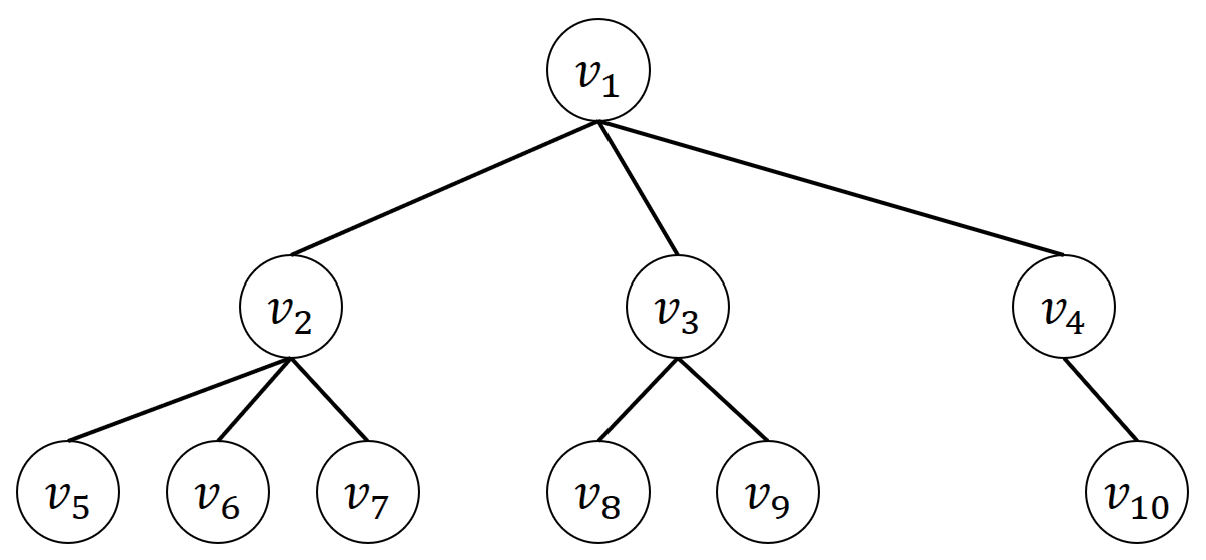
\includegraphics[width=0.5\textwidth]{figures/0.eps}\\
  \caption{depth-first and breadth-first tree}\label{figure_0}
\end{figure}
We firstly focus on breadth-first search tree.
We note two vertexes in the same layer(BFS search tree) and satisfy $v_i$ is before $v_j$ as $v_i \prec v_j$. We note prt($v$) as the parent node of $v$. Supposed that there is an edge $e$ which is not belong to $T$, then $e$ cannot across two or more layers in $T$. And $e$ cannot be $(\textrm{prt}(u),v)$ satisfying prt($u$) $\neq$ prt($v$) and $u\prec v$. Then $e$ must be the edge of the two following cases:

1) $e$ is between two vertexes $v_i$ and $v_j$ satisfying prt($v_i$)=prt($v_j$). As show in figure~\ref{figure_1_2}, in this case, the DFS tree is different from the BFS tree because $v_7$ will be access as the son of $v_6$ not the son of $v_2$ in the BFS tree.
\begin{figure}[!htbp]
\centering
\subfigure[BFS]{
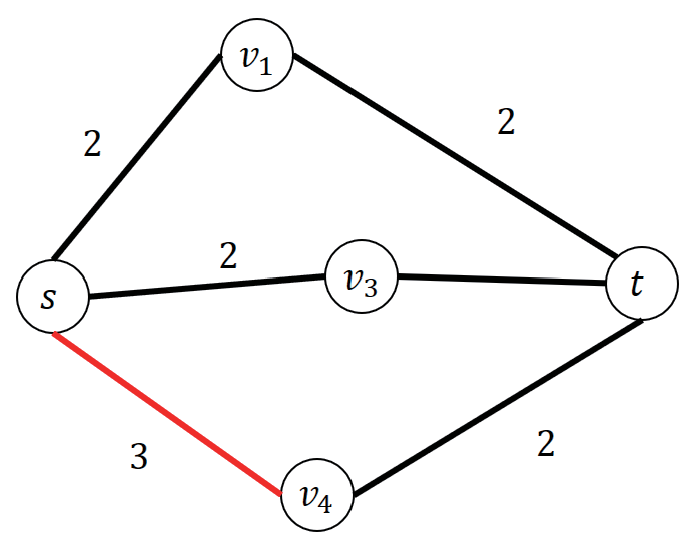
\includegraphics[width=0.3\textwidth]{figures/1.eps}}
\subfigure[DFS]{
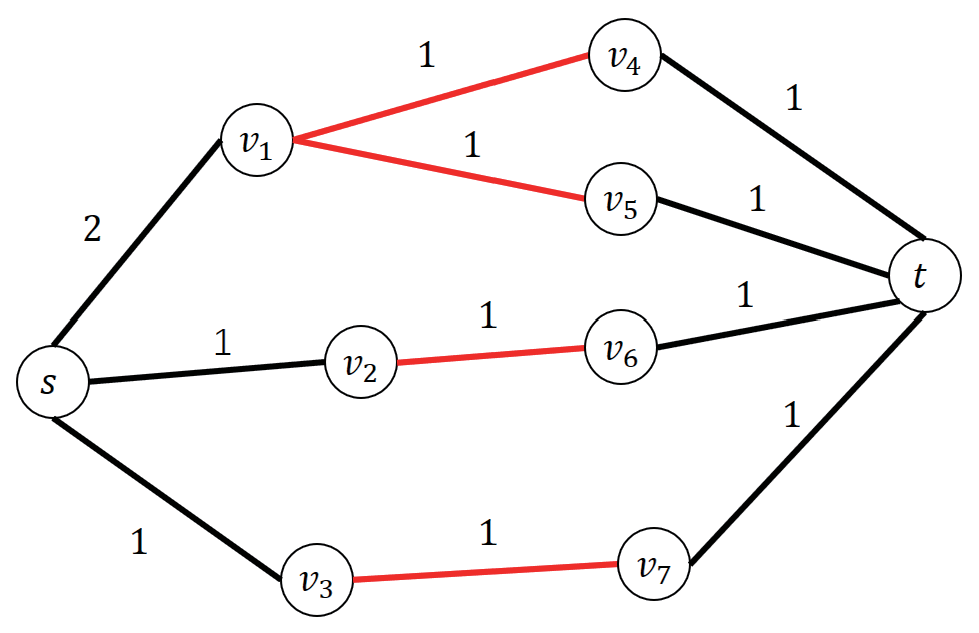
\includegraphics[width=0.3\textwidth]{figures/2.eps}}
\caption{$e$ is between two vertexes $v_i$ and $v_j$ satisfying prt($v_i$)=prt($v_j$)}\label{figure_1_2}
\end{figure}

2) $e$ is between two vertexes $v_i$ and $v_j$ satisfying prt($v_i$) $\neq$ prt($v_j$) and $v_j\prec v_i$. As show in figure~\ref{figure_3_4}, in this case, the DFS tree is different from the BFS tree because $v_3$ will be access as the son of $v_7$ not the son of $v_1$ in the BFS tree.
\begin{figure}[!htbp]
\centering
\subfigure[BFS]{
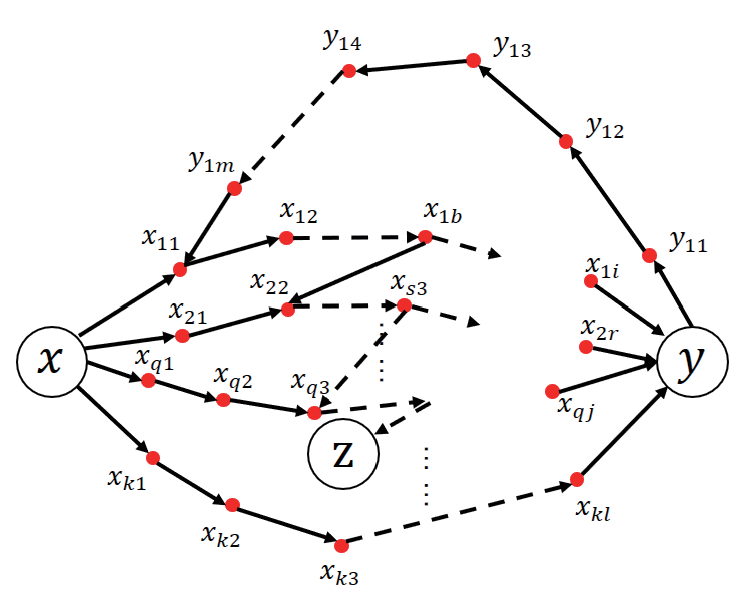
\includegraphics[width=0.3\textwidth]{figures/3.eps}}
\subfigure[DFS]{
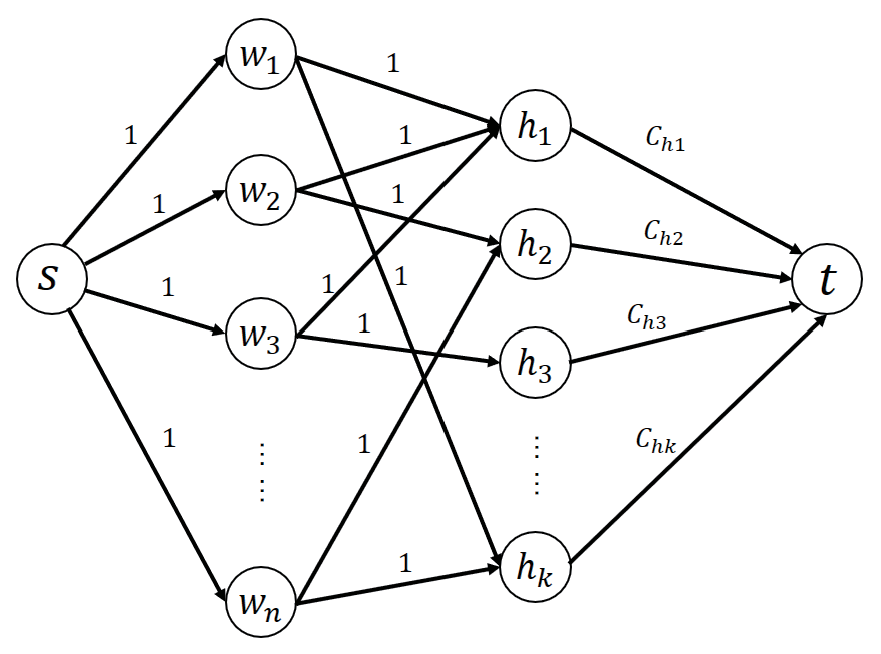
\includegraphics[width=0.3\textwidth]{figures/4.eps}}
\caption{$e$ is between two vertexes $v_i$ and $v_j$ satisfying prt($v_i$) $\neq$ prt($v_j$) and $v_j\prec v_i$}\label{figure_3_4}
\end{figure}


%% !Mode:: "TeX:UTF-8"

\chapter{}
\textbf{
There's a natural intuition that two nodes that are far apart in a communication network——separated by many hops——have a more tenuous connection than two nodes that are close together. There are a number of algorithmic results that are based to some extent on different ways of making this notion precise. Here's one that involves the susceptibility of paths to the deletion of nodes.
}

\textbf{
Suppose that an $n$-node undirected graph $G=(V,E)$ contains two nodes $s$ and $t$ such that the distance between $s$ and $t$ is strictly greater than $n/2$. Show that there must exist some node $v$, not equal to either $s$ or $t$, such that deleting $v$ from $G$ destroys all $s-t$ paths.(In other words, the graph obtained from $G$ by deleting $v$ contains no path from $s$ to $t$.) Give an algorithm with running time $O(m+n)$ to find such a node $v$.
}

\hspace*{\fill} \\

According to BFS algorithm and the given conditions, as shown in figure~\ref{figure_5_1}, there exists an separated layers satisfying that the count of layers is $m$ and $m-1> n/2 $. The problem is equal to Pigeon nest problem. Notice that there remain at most $n-2$ vertexes which will be put into $m-1$ cells. And notice that $2(m-1)>n>n-2$. So there must be at least one cell(actually two cells) that contains only one vertex. That is to say there exists some node $v$ that satisfying our goal.
\begin{figure}[!htbp]
  \centering
  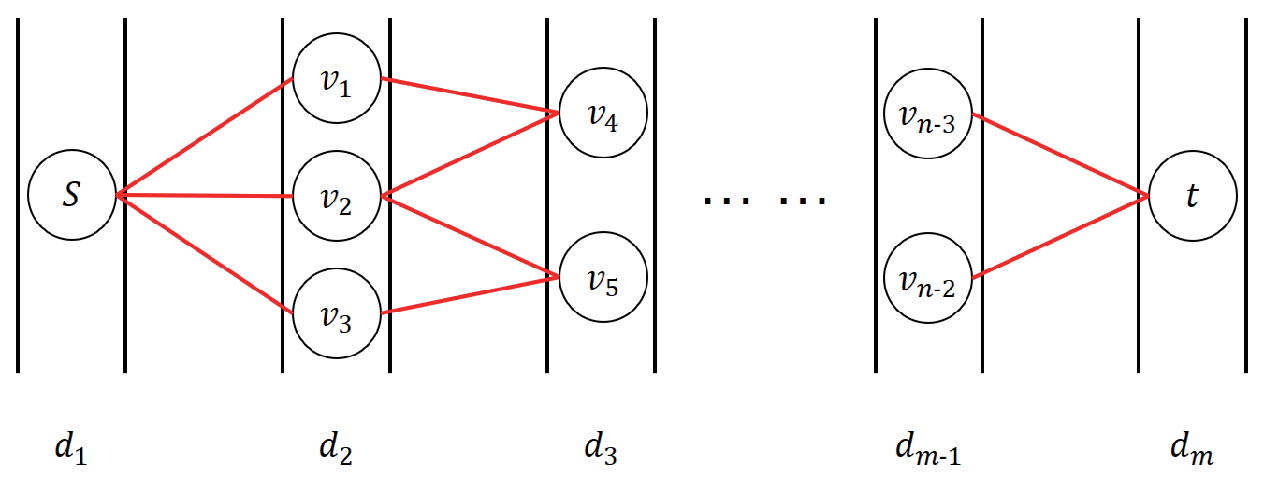
\includegraphics[width=0.7\textwidth]{figures/5_1.eps}\\
  \caption{The layers of breadth-first search}\label{find_key_point}
\end{figure}

We next give an algorithm to find one of these vertex. Generally speaking, we just need to execute depth-first traversal rooted at $S$ and get tree $T$. Because $s$ and $t$ are connected, $t$ is definitely in $T$. Besides, it is sure that there is at leat one layer that contains one vertex. So we just need to find this vertex. We give the detail process in Alg~\ref{find_key_point}.

\begin{algorithm}[!htbp]
\caption{The pivotal vertex discovering}
\label{find_key_point}
\begin{algorithmic}[1]
\REQUIRE $s$
\STATE{Set Discovered[$s$]=$true$ and Discovered[$v$]=$false$ for all other $v$}
\STATE{Initialize $L[0]$ to consist of the single element $s$}
\STATE{Set the layer count $i$=0}
\STATE{Set result node rnode = $null$}
\WHILE{$L[i]\neq \phi$}
    \IF{Size($L[i]$) = 1 and $i>0$}
        \STATE{Set rnode = $L[i][0]$}
        \STATE{break}
    \ENDIF
    \STATE{Initialize an empty list L[$i+1$]}
    \FOR{each node $u\in L[i]$}
        \STATE{Consider each edge $(u,v)$ incident to $u$}
        \IF{Discovered[$v$]=$false$}
            \STATE{Set Discovered[$v$]=$true$}
            \STATE{Add $v$ to the list $L[i+1]$}
        \ENDIF
    \ENDFOR
    \STATE{Increment the layer counter $i$ by one}
\ENDWHILE   
\STATE Return rnode
\end{algorithmic}
\end{algorithm}

As showed in Alg~\ref{find_key_point}, we test the number of each layer(line 6). When the count of layer number is one and it is not the first layer, we set the result node as the single element in this layer and break the loop.


%%%%%%%%%% 正文部分内容  %%%%%%%%%%

\clearpage
\end{CJK*}                                        % 结束中文字体使用
\end{document}                                    % 结束全文
